\documentclass[tikz,border=10pt]{standalone}
\usetikzlibrary{arrows.meta, positioning, shapes.geometric}

\begin{document}
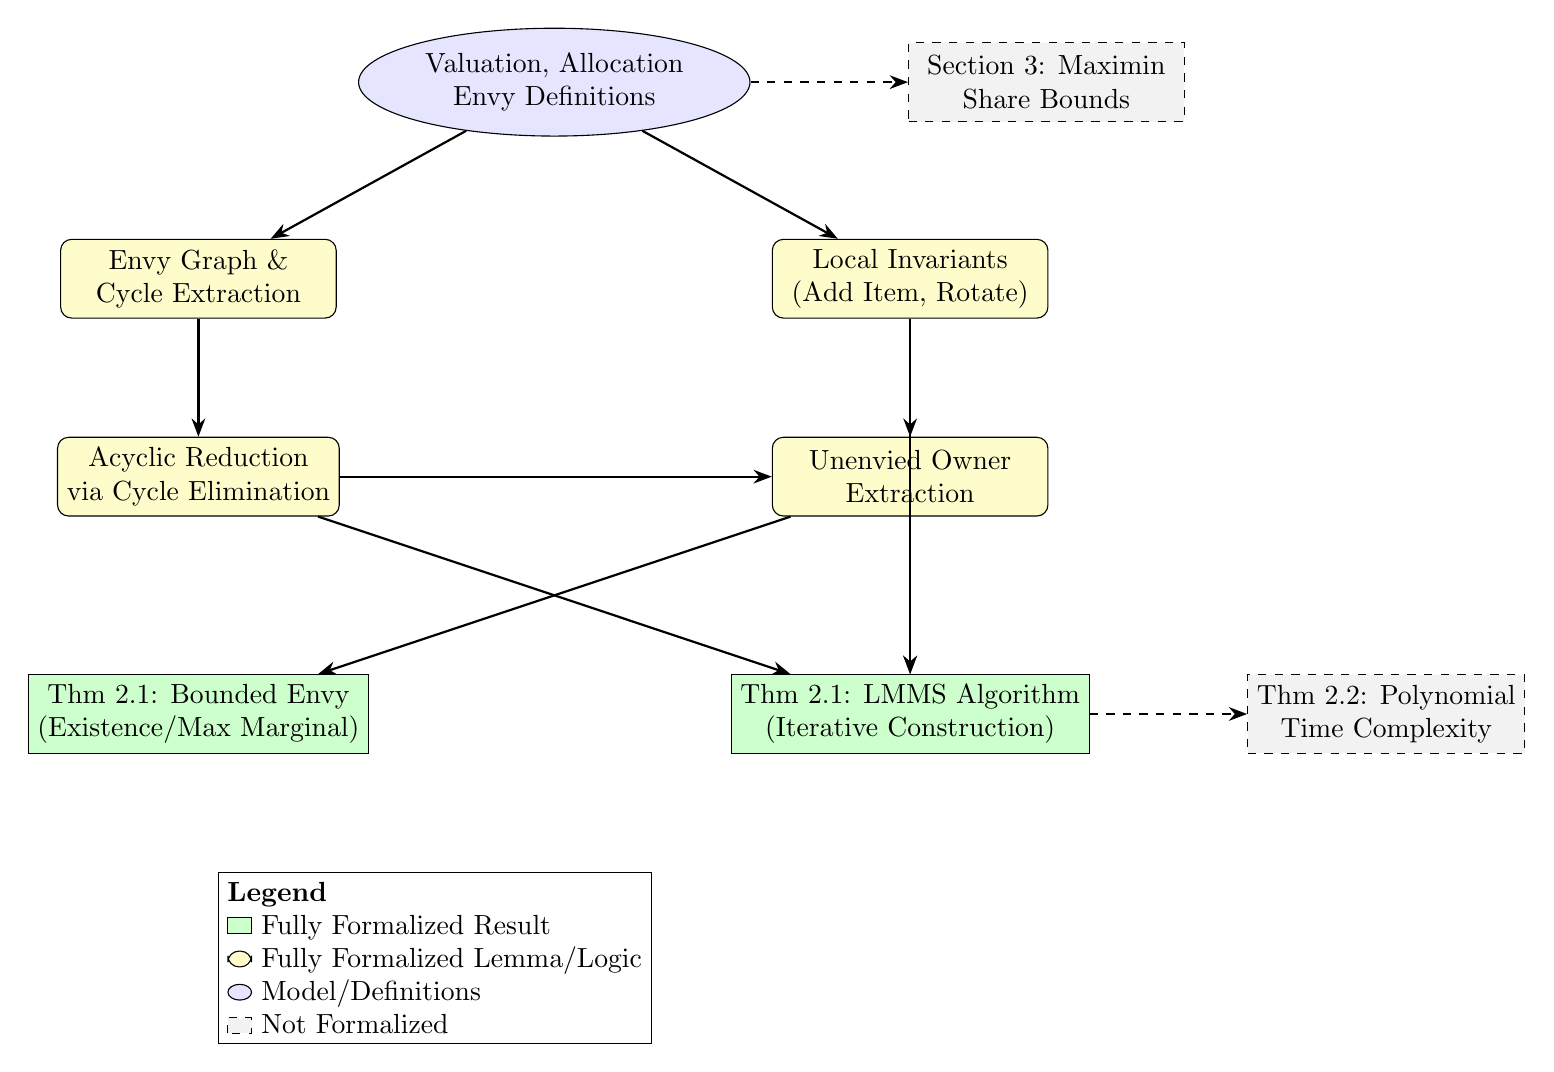
\begin{tikzpicture}[
    node distance=1.5cm and 1cm,
    result/.style={rectangle, draw, fill=green!20, minimum width=3.5cm, minimum height=1cm, align=center},
    model/.style={ellipse, draw, fill=blue!10, minimum width=3cm, minimum height=1cm, align=center},
    lemma/.style={rectangle, draw, fill=yellow!20, minimum width=3.5cm, minimum height=1cm, align=center, rounded corners},
    unformalized/.style={rectangle, draw, dashed, fill=gray!10, minimum width=3.5cm, minimum height=1cm, align=center},
    arrow/.style={-{Stealth}, thick}
]

% Center Column (Definitions)
\node[model] (Primitives) {Valuation, Allocation \\ Envy Definitions};

% Left Column (Graph/Acyclic)
\node[lemma, below left=1.5cm and 1cm of Primitives] (Graph) {Envy Graph \& \\ Cycle Extraction};
\node[lemma, below=of Graph] (Acyclic) {Acyclic Reduction \\ via Cycle Elimination};

% Right Column (Local/Unenvied)
\node[lemma, below right=1.5cm and 1cm of Primitives] (Local) {Local Invariants \\ (Add Item, Rotate)};
\node[lemma, below=of Local] (Unenvied) {Unenvied Owner \\ Extraction};

% Results
\node[result, below=2cm of Acyclic] (ThmExist) {Thm 2.1: Bounded Envy \\ (Existence/Max Marginal)};
\node[result, below=2cm of Unenvied] (ThmAlgo) {Thm 2.1: LMMS Algorithm \\ (Iterative Construction)};

% Unformalized
\node[unformalized, right=2cm of ThmAlgo] (Thm2_2) {Thm 2.2: Polynomial \\ Time Complexity};
\node[unformalized, right=2cm of Primitives] (Sec3) {Section 3: Maximin \\ Share Bounds};

% Edges
\draw[arrow] (Primitives) -- (Graph);
\draw[arrow] (Primitives) -- (Local);
\draw[arrow] (Graph) -- (Acyclic);
\draw[arrow] (Local) -- (Unenvied);
\draw[arrow] (Acyclic) -- (Unenvied);
\draw[arrow] (Unenvied) -- (ThmExist);
\draw[arrow] (Unenvied) -- (ThmAlgo);
\draw[arrow] (Local) -- (ThmAlgo);
\draw[arrow] (Acyclic) -- (ThmAlgo);

% Edges to Unformalized
\draw[arrow, dashed] (ThmAlgo) -- (Thm2_2);
\draw[arrow, dashed] (Primitives) -- (Sec3);

% Legend
\node[draw, rectangle, below=1.5cm of ThmExist, xshift=3cm, align=left] (Legend) {
    \textbf{Legend} \\
    \tikz\draw[fill=green!20] (0,0) rectangle (0.3,0.2); Fully Formalized Result \\
    \tikz\draw[fill=yellow!20, rounded corners] (0,0) rectangle (0.3,0.2); Fully Formalized Lemma/Logic \\
    \tikz\draw[fill=blue!10] (0,0) ellipse (0.15 and 0.1); Model/Definitions \\
    \tikz\draw[dashed, fill=gray!10] (0,0) rectangle (0.3,0.2); Not Formalized
};

\end{tikzpicture}
\end{document}